\chapter{Lindenmayer-Systeme}

Vorstellung der verwendeten Konzepte.

\section{Kontextfreie Grammatik}

Bei L-Systemen handelt es sich um, auf Zeichenketten basierende, Ersetzungssysteme. Es werden komplexe Objekte beschrieben, indem Teile der Zeichenkette durch andere Zeichen oder Zeichenketten ersetzt werden. Die Beschreibung dieser Ersetzungen findet mittels festgelegter Produktionsregeln statt. \cite[S.2]{ABOP:04} 

Eine formale Definition eines auf Zeichenketten arbeitenden Ersetzungssystems wird durch kontextfreie Grammatiken gegeben:

\newtheorem{defKontextfreieGrammatik}{Kontextfreie Grammatik:}[chapter]
\begin{defKontextfreieGrammatik}
	Eine kontextfreie Grammatik G ist ein Tupel G = $(V, N, P, \omega)$ bestehend aus:
	\begin{enumerate}
		\item $V$ -- einer nichtleeren, endlichen Menge von Buchstaben (Alphabet).
		\item $N$ -- einer endlichen Menge von Variablen.
		\item $P$ -- einer endlichen Menge von Produktionsregeln in der Form $P: A \rightarrow \alpha$ mit $A \in N$ und $\alpha \in (V \cup N )^*$.
		\item $\omega \in N$ -- dem Axiom, Startsymbol der Grammatik.
	\end{enumerate}
	\cite[S.343]{ThI:14}
\end{defKontextfreieGrammatik}

Die Menge $V^*$ ist die Menge aller Wörter über $V$ -- die Menge aller Wörter, die aus dem Alphabet $V$ gebildet werden können. \cite[S.70]{ThI:14} 

Eine Grammatik wird als kontextfrei bezeichnet, wenn beispielsweise die Produktionsregel $A \rightarrow \alpha$ angewendet werden kann, ohne die $A$ umgebenden Buchstaben -- seinen Kontext -- beachten zu müssen. \cite[S.343]{ThI:14} 

Eine Grammatik wird als deterministisch bezeichnet, wenn es genau eine Produktionsregel $r \in P$ für jede Variable $A \in V$ gibt, sodass $r: A \rightarrow \alpha$, $\alpha \in (V \cup N )^*$. Das bedeutet, dass die Ersetzung einer Variable eindeutig durch eine einzige Regel beschrieben wird. \cite[S.75]{PCGiG:16}

Die Anwendung der Produktionsregeln findet meist sequentiell statt -- die Zeichenkette wird von links nach rechts durchlaufen und Ersetzungen werden direkt auf die untersuchte Zeichenkette angewendet. \cite[S.75]{PCGiG:16}

\section{D0L-Systeme}

Diese Arbeit beschränkt sich auf die Behandlung deterministischer, kontextfreier L-Systeme, auch D0L-Systeme genannt. Diese besitzen die Eigenschaften einer deterministischen und kontextfreien Grammatik, Produktionsregeln werden jedoch parallel und gleichzeitig auf alle Buchstaben des untersuchten Wortes angewendet. Dieses Vorgehen soll die Zellteilung in mehrzelligen Organismen simulieren und ist somit an biologische Vorgänge angelehnt. \cite[S. 3]{ABOP:04} 

Ein D0L-System kann wie folgt definiert werden:
\newtheorem{defD0LSystem}{D0L-System:}[chapter]
\begin{defD0LSystem}
	Ein D0L-System ist ein Tupel G = $(V, P, \omega)$, bestehend aus
	\begin{enumerate}
		\item $V$ -- einem nichtleeren, endlichen Alphabet.
		\item $P$ -- einer endlichen Menge von Produktionsregeln in der Form $P: a \rightarrow b$ mit $a \in V$ und $b \in V^*$. $a$ wird als Vorgänger, $b$ als Nachfolger bezeichnet. Ist für einen Buchstaben $x \in V$ keine explizite Produktionsregel angegeben, wird die Identitätsproduktion $P: x \rightarrow x$ angenommen -- der Buchstabe wird durch sich selbst ersetzt.
		\item $\omega \in V^+$ -- dem Axiom, Startsymbol der Grammatik.
	\end{enumerate}
Die Menge $V^+$ ist die Menge aller nichtleeren Wörter über $V$. \cite[S.4]{ABOP:04} 
\end{defD0LSystem}

Die Ableitung eines Wortes entspricht der Ersetzung aller Buchstaben anhand der Produktionsregeln. Ein Wort kann mehrmals abgeleitet werden. 

\newtheorem{defAbleitung}{Ableitung:}[chapter]
\begin{defAbleitung}
	Gegeben sei ein Wort $w = a_1 ... a_m$ mit $w \in V^*$ und $a_i \in V^*$. Das Wort $v = b_1 ... b_m$ mit $v \in V^*$ und $b_i \in V^*$ ist die Ableitung von $w$ wenn für alle $i=1...m$ eine Produktionsregel $a_i \rightarrow b_i$ existiert. Die Ableitung wird als $w \Rightarrow v$ notiert. \\
	Das Wort $w_n$ ist die n-te Ableitung des Wortes $w_0$ wenn eine Folge von Wörtern $w_0, w_1, ..., w_n$ mit Ableitungen $w_0 \Rightarrow w_1 \Rightarrow ... \Rightarrow w_n$ existiert. \cite[S.4]{ABOP:04} 
\end{defAbleitung}

\paragraph{Anabaena}

Beispiel: Das Wachstum der Blaualgen-Gattung \glqq Anabaena\grqq{} kann durch ein L-System simuliert werden. Die Buchstaben $a$ und $b$ beschreiben die Größe und Teilungsbereitschaft einer Algenzelle, während die Indizes $l$ und $r$ die Polarität einer Zelle darstellen. Es gelten folgende Produktionsregeln:
\begin{equation}
\begin{array}{cccc}
 p_1 & : a_r &\rightarrow& a_lb_r \\
p_2 &  : a_l &\rightarrow& b_la_r \\ 
p_3 &  : b_r &\rightarrow& a_r \\
p_4 &  : b_l &\rightarrow& a_l 
\end{array}
\label{eq:ProdAnabaena}
\end{equation} 

Die Entwicklung einer Anfangszelle $a_r$ (Axiom $\omega : a_r$) läuft daraufhin wie in Abbildung \ref{fig:AnabaenaAbleitung} dargestellt ab.
\begin{figure} [hbtp]
	\centering
	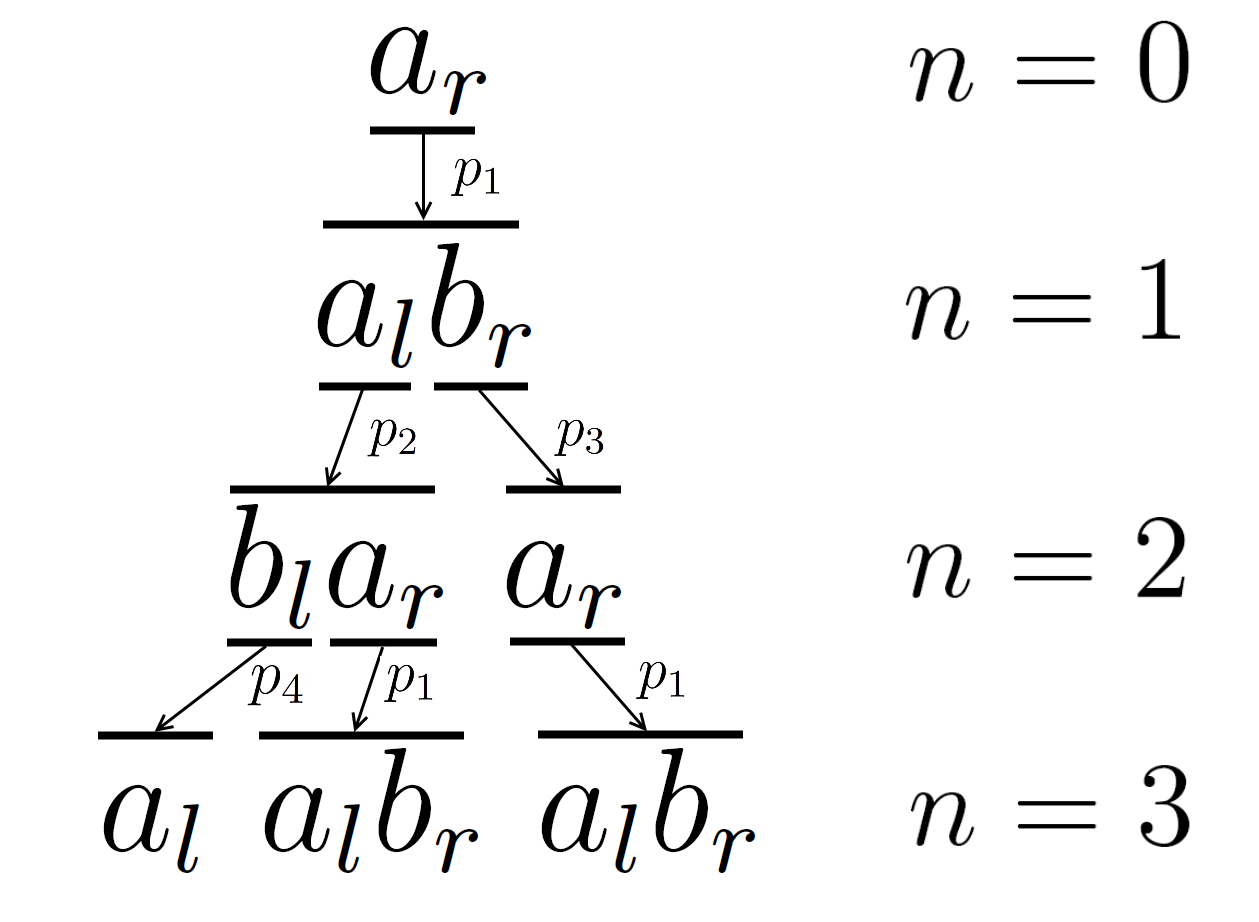
\includegraphics[height=0.3\textheight]{images/AnabaenaAbleitung.png}
	\caption{n-fache Ableitung der Anfangszelle $a_r$ anhand der Produktionsregeln $p_1 ... p_4$ aus Gleichung \ref{eq:ProdAnabaena}. Eigene Abbildung anhand \cite[S.4]{ABOP:04}}
	\label{fig:AnabaenaAbleitung}
\end{figure}

\subsection{Parametrische L-Systeme}

Parametrische L-Systeme stellen eine Erweiterung der D0L-Systeme dar. Die Buchstaben eines verwendeten Alphabets $V$ werden um zugeordnete Parameter aus der Menge der reelen Zahlen ergänzt. Ein solches parametrisches Wort $V \times \Re^*$ besteht aus einem Zeichen $A \in V$ und Parametern $a_1,...,a_n \in \Re$ und wird als $A(a_1,...,a_n)$ dargestellt. Ein parametrisches Wort ohne Parameter mit dem Zeichen $A \in V$  wird schlicht als $A$ dargestellt. \cite[S.41]{ABOP:04}

Während in der Definition von Modulen numerische Konstanten verwendet werden, werden bei der Angabe eines L-Systems Variablen verwendet. Ist $\Sigma$ eine Menge von Variablen, dann ist $E(\Sigma)$ ein arithmetischer Ausdruck, in dem Variablen, Konstanten und arithmetische Operatoren auf eine zulässige Weise kombiniert werden. \cite[S.41]{ABOP:04}

\newtheorem{defParametrischeLSysteme}{Parametrisches L-System:}[section]
\begin{defParametrischeLSysteme}
	Ein Parametrisches L-System ist ein Tupel G = $(V, \Sigma, P, \omega)$, bestehend aus
	\begin{enumerate}
		\item $V$ -- einem nichtleeren, endlichen Alphabet.
		\item $\Sigma$ -- einer Menge der Variablen.
		\item $P$ -- einer endlichen Menge von Produktionsregeln $P : (V\times \Sigma^*) \rightarrow (V\times E(\Sigma))^*$
		\item $\omega \in M^+$ mit $M =(V \times \Re^*)$ -- einem Axiom in Form eines nichtleeren, parametrischen Wortes.
	\end{enumerate}
\cite[S.41]{ABOP:04}
\end{defParametrischeLSysteme}

Eine Produktion kann auf ein parametrisches Wort angewendet werden wenn das Zeichen, das dem Wort vorausgeht, und die Anzahl der Parameter mit dem Zeichen und der Anzahl der Parameter im Vorgänger der Produktionsregel übereinstimmen. \cite[S.42]{ABOP:04}

Beispiel: Gegeben sei folgendes, parametrisches L-System:

\begin{equation}
\begin{array}{llll}
\omega & : A(1,1) \\
p_1 & : A(x,y) &\rightarrow& A(x+1, y*2)\text{ }B(y) \\
p_2 &  : B(x) &\rightarrow& B(x+1)\text{ }C 
\end{array}
\label{eq:ProdParamLSystem}
\end{equation} 

Das Alphabet $V$ und die Menge der Variablen $\Sigma$ gehen implizit aus der Angabe der Produktionsregeln hervor. Die Entwicklung des L-Systems läuft anhand Abbildung \ref{fig:ParamLSystemBeispiel} ab. 

\begin{figure} [hbtp]
	\centering
	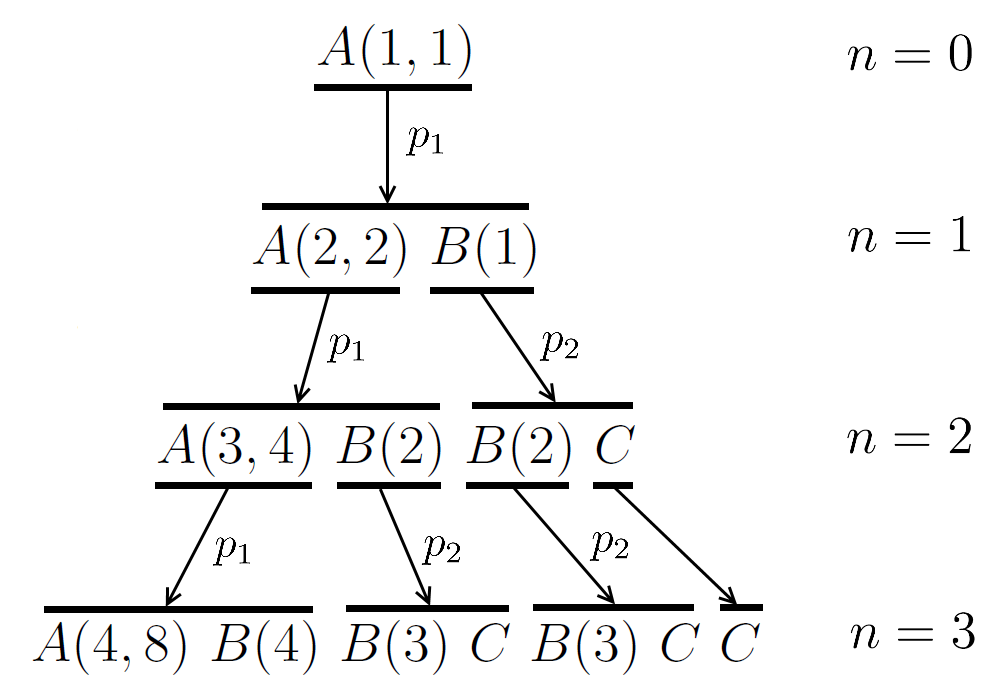
\includegraphics[height=0.4\textheight]{images/ParamLSystemBeispiel.png}
	\caption{n-fache Ableitung des Axioms $A(1,1)$ anhand der Produktionsregeln aus Gleichung \ref{eq:ProdParamLSystem}. Die Ersetzung des Zeichens $C$ erfolgt anhand der impliziten Identitätsproduktion. Eigene Abbildung.}
	\label{fig:ParamLSystemBeispiel}
\end{figure}

\section{Grafische Interpretation von L-Systemen}

Um die Ergebnisse von L-Systemen in Form von 3D-Objekten zu visualisieren, muss eine grafische Interpretation der resultierenden Zeichenketten festgelegt werden. Im Folgenden wird die verwendete Visualisierungsmethode, Turtle-Interpretation, vorgestellt.

\subsection{Turtle-Interpretation}

Die Turtle-Interpretation entspricht einer 

\subsection{Verzweigte L-Systeme}
asd
\section{L-Systeme für Baumstrukturen}
asd
